\documentclass[12pt,table,t]{beamer}

% Packages
\usepackage{xcolor}
\usepackage{eulervm}
\usepackage[utf8]{inputenc}


% Theme
\mode<presentation>
{
  \usetheme{Honefoss}
%  \setbeamercovered{transparent}
  \setbeamertemplate{blocks}[rounded]
  \AtBeginPart{\frame[c]{\partpage}}
}

\newcommand{\comment}[1]{{\slshape\color{kvred}#1}}
\newcommand{\Where}[0]{\textbf{Where} }
\newcommand{\Midgard}[0]{\textbf{Midgard} }
\newcommand{\Asgard}[0]{\textbf{Åsgard} }

\usepackage{bbding}
\newcommand{\yes}{{\color{kvgreen}\CheckmarkBold}}
\newcommand{\no}{{\color{kvred}\XSolidBold}}

% Quotes (https://tex.stackexchange.com/questions/365231/enclose-a-custom-quote-environment-in-quotes-from-csquotes)
\usepackage[style=british]{csquotes}
\def\signed #1{{\leavevmode\unskip\nobreak\hfil\penalty50\hskip1em
  \hbox{}\nobreak\hfill #1%
  \parfillskip=0pt \finalhyphendemerits=0 \endgraf}}
\newsavebox\mybox
\newenvironment{aquote}[1]
  {\savebox\mybox{#1}\begin{quote}\openautoquote\hspace*{-.7ex}}
  {\unskip\closeautoquote\vspace*{1mm}\signed{\usebox\mybox}\end{quote}}

\usepackage{fancyvrb}
\newcommand{\VerbBar}{|}
\newcommand{\VERB}{\Verb[commandchars=\\\{\}]}
\DefineVerbatimEnvironment{Highlighting}{Verbatim}{commandchars=\\\{\}}
% Add ',fontsize=\small' for more characters per line
\newenvironment{Shaded}{}{}
\newcommand{\KeywordTok}[1]{\tiny\textcolor[rgb]{0.00,0.44,0.13}{\textbf{#1}}}
\newcommand{\DataTypeTok}[1]{\tiny\textcolor[rgb]{0.56,0.13,0.00}{#1}}
\newcommand{\DecValTok}[1]{\tiny\textcolor[rgb]{0.25,0.63,0.44}{#1}}
\newcommand{\BaseNTok}[1]{\tiny\textcolor[rgb]{0.25,0.63,0.44}{#1}}
\newcommand{\FloatTok}[1]{\tiny\textcolor[rgb]{0.25,0.63,0.44}{#1}}
\newcommand{\ConstantTok}[1]{\tiny\textcolor[rgb]{0.53,0.00,0.00}{#1}}
\newcommand{\CharTok}[1]{\tiny\textcolor[rgb]{0.25,0.44,0.63}{#1}}
\newcommand{\SpecialCharTok}[1]{\tiny\textcolor[rgb]{0.25,0.44,0.63}{#1}}
\newcommand{\StringTok}[1]{\tiny\textcolor[rgb]{0.25,0.44,0.63}{#1}}
\newcommand{\VerbatimStringTok}[1]{\tiny\textcolor[rgb]{0.25,0.44,0.63}{#1}}
\newcommand{\SpecialStringTok}[1]{\tiny\textcolor[rgb]{0.73,0.40,0.53}{#1}}
\newcommand{\ImportTok}[1]{\tiny#1}
\newcommand{\CommentTok}[1]{\tiny\textcolor[rgb]{0.38,0.63,0.69}{\textit{#1}}}
\newcommand{\DocumentationTok}[1]{\tiny\textcolor[rgb]{0.73,0.13,0.13}{\textit{#1}}}
\newcommand{\AnnotationTok}[1]{\tiny\textcolor[rgb]{0.38,0.63,0.69}{\textbf{\textit{#1}}}}
\newcommand{\CommentVarTok}[1]{\tiny\textcolor[rgb]{0.38,0.63,0.69}{\textbf{\textit{#1}}}}
\newcommand{\OtherTok}[1]{\tiny\textcolor[rgb]{0.00,0.44,0.13}{#1}}
\newcommand{\FunctionTok}[1]{\tiny\textcolor[rgb]{0.02,0.16,0.49}{#1}}
\newcommand{\VariableTok}[1]{\tiny\textcolor[rgb]{0.10,0.09,0.49}{#1}}
\newcommand{\ControlFlowTok}[1]{\tiny\textcolor[rgb]{0.00,0.44,0.13}{\textbf{#1}}}
\newcommand{\OperatorTok}[1]{\tiny\textcolor[rgb]{0.40,0.40,0.40}{#1}}
\newcommand{\BuiltInTok}[1]{\tiny#1}
\newcommand{\ExtensionTok}[1]{\tiny#1}
\newcommand{\PreprocessorTok}[1]{\tiny\textcolor[rgb]{0.74,0.48,0.00}{#1}}
\newcommand{\AttributeTok}[1]{\tiny\textcolor[rgb]{0.49,0.56,0.16}{#1}}
\newcommand{\RegionMarkerTok}[1]{\tiny#1}
\newcommand{\InformationTok}[1]{\tiny\textcolor[rgb]{0.38,0.63,0.69}{\textbf{\textit{#1}}}}
\newcommand{\WarningTok}[1]{\tiny\textcolor[rgb]{0.38,0.63,0.69}{\textbf{\textit{#1}}}}
\newcommand{\AlertTok}[1]{\tiny\textcolor[rgb]{1.00,0.00,0.00}{\textbf{#1}}}
\newcommand{\ErrorTok}[1]{\tiny\textcolor[rgb]{1.00,0.00,0.00}{\textbf{#1}}}
\newcommand{\NormalTok}[1]{\tiny#1}
\usepackage{graphicx,grffile}
\makeatletter
\def\maxwidth{\ifdim\Gin@nat@width>\linewidth\linewidth\else\Gin@nat@width\fi}
\def\maxheight{\ifdim\Gin@nat@height>\textheight0.8\textheight\else\Gin@nat@height\fi}
\makeatother
% Scale images if necessary, so that they will not overflow the page
% margins by default, and it is still possible to overwrite the defaults
% using explicit options in \includegraphics[width, height, ...]{}
\setkeys{Gin}{width=\maxwidth,height=\maxheight,keepaspectratio}

% Set up a framed environment for code snippets
%\usepackage[scaled]{beramono}
\usepackage[framemethod=default]{mdframed}
\usepackage{listings}
\lstset{basicstyle=\scriptsize\sffamily\color{kvblue},breaklines=true,%
  showstringspaces=false,commentstyle=\color{kvred},columns=flexible,%
  stringstyle=\color{kvgreen},escapeinside={(*@}{@*)},numbers=left,%
  numbersep=1em,numberstyle=\tiny\sffamily\color{kvlightblue},%
  xleftmargin=2em,inputencoding=utf8,extendedchars=true,%
  literate={æ}{{\ae}}1 {ø}{{\o}}1 {å}{{\aa}}1 {Æ}{{\AE}}1 {Ø}{{\O}}1 {Å}{{\AA}}1 }
\global\mdfdefinestyle{notedefault}{%
nobreak=true,linecolor=kvgreen,linewidth=1pt,%
outermargin=.3cm,innermargin=.3cm,innertopmargin=-1ex,skipabove=2ex,skipbelow=2cm,%
shadow=true,shadowcolor=black!20,shadowsize=4pt,%
}
\newenvironment{notetwo}[1]{%
  \mdfsetup{%
    frametitle={\colorbox{white}{\,\textsc{\color{kvred}#1}\,}},
    frametitleaboveskip=-.75\ht\strutbox,
    frametitlealignment=\raggedright
  }%
  \mdframed[style=notedefault]
}{\endmdframed\bigskip}

\lstnewenvironment{lsttermcmd}{\notetwo{Terminal}\lstset{morecomment=[l][keywordstyle]{>},morecomment=[l][commentstyle]{\#}}}{\endnotetwo}
\lstnewenvironment{lstpython}{\notetwo{Python}\lstset{language=python}}{\endnotetwo}
\lstnewenvironment{lstpycon}{\notetwo{Python}\lstset{language=python,numbers=none,xleftmargin=0em,literate={æ}{{\ae}}1 {ø}{{\o}}1 {å}{{\aa}}1 {Æ}{{\AE}}1 {Ø}{{\O}}1 {Å}{{\AA}}1 {>>>}{{\textgreater\kern-.4em\textgreater\kern-.4em\textgreater\kern.4em}}1 }}{\endnotetwo}
\lstnewenvironment{lstoutput}{\notetwo{}\lstset{basicstyle=\tiny\color{kvgreen},numbers=none,xleftmargin=0em}}{\endnotetwo}


\title{Where, Midgard og Åsgard}
\author{Geir~Arne~Hjelle \and Michael~D\"ahnn \and Ann-Silje~Kirkvik \and Ingrid~Fausk}
\date{Frokostmøte, 6.\ desember 2018}
\titlegraphic{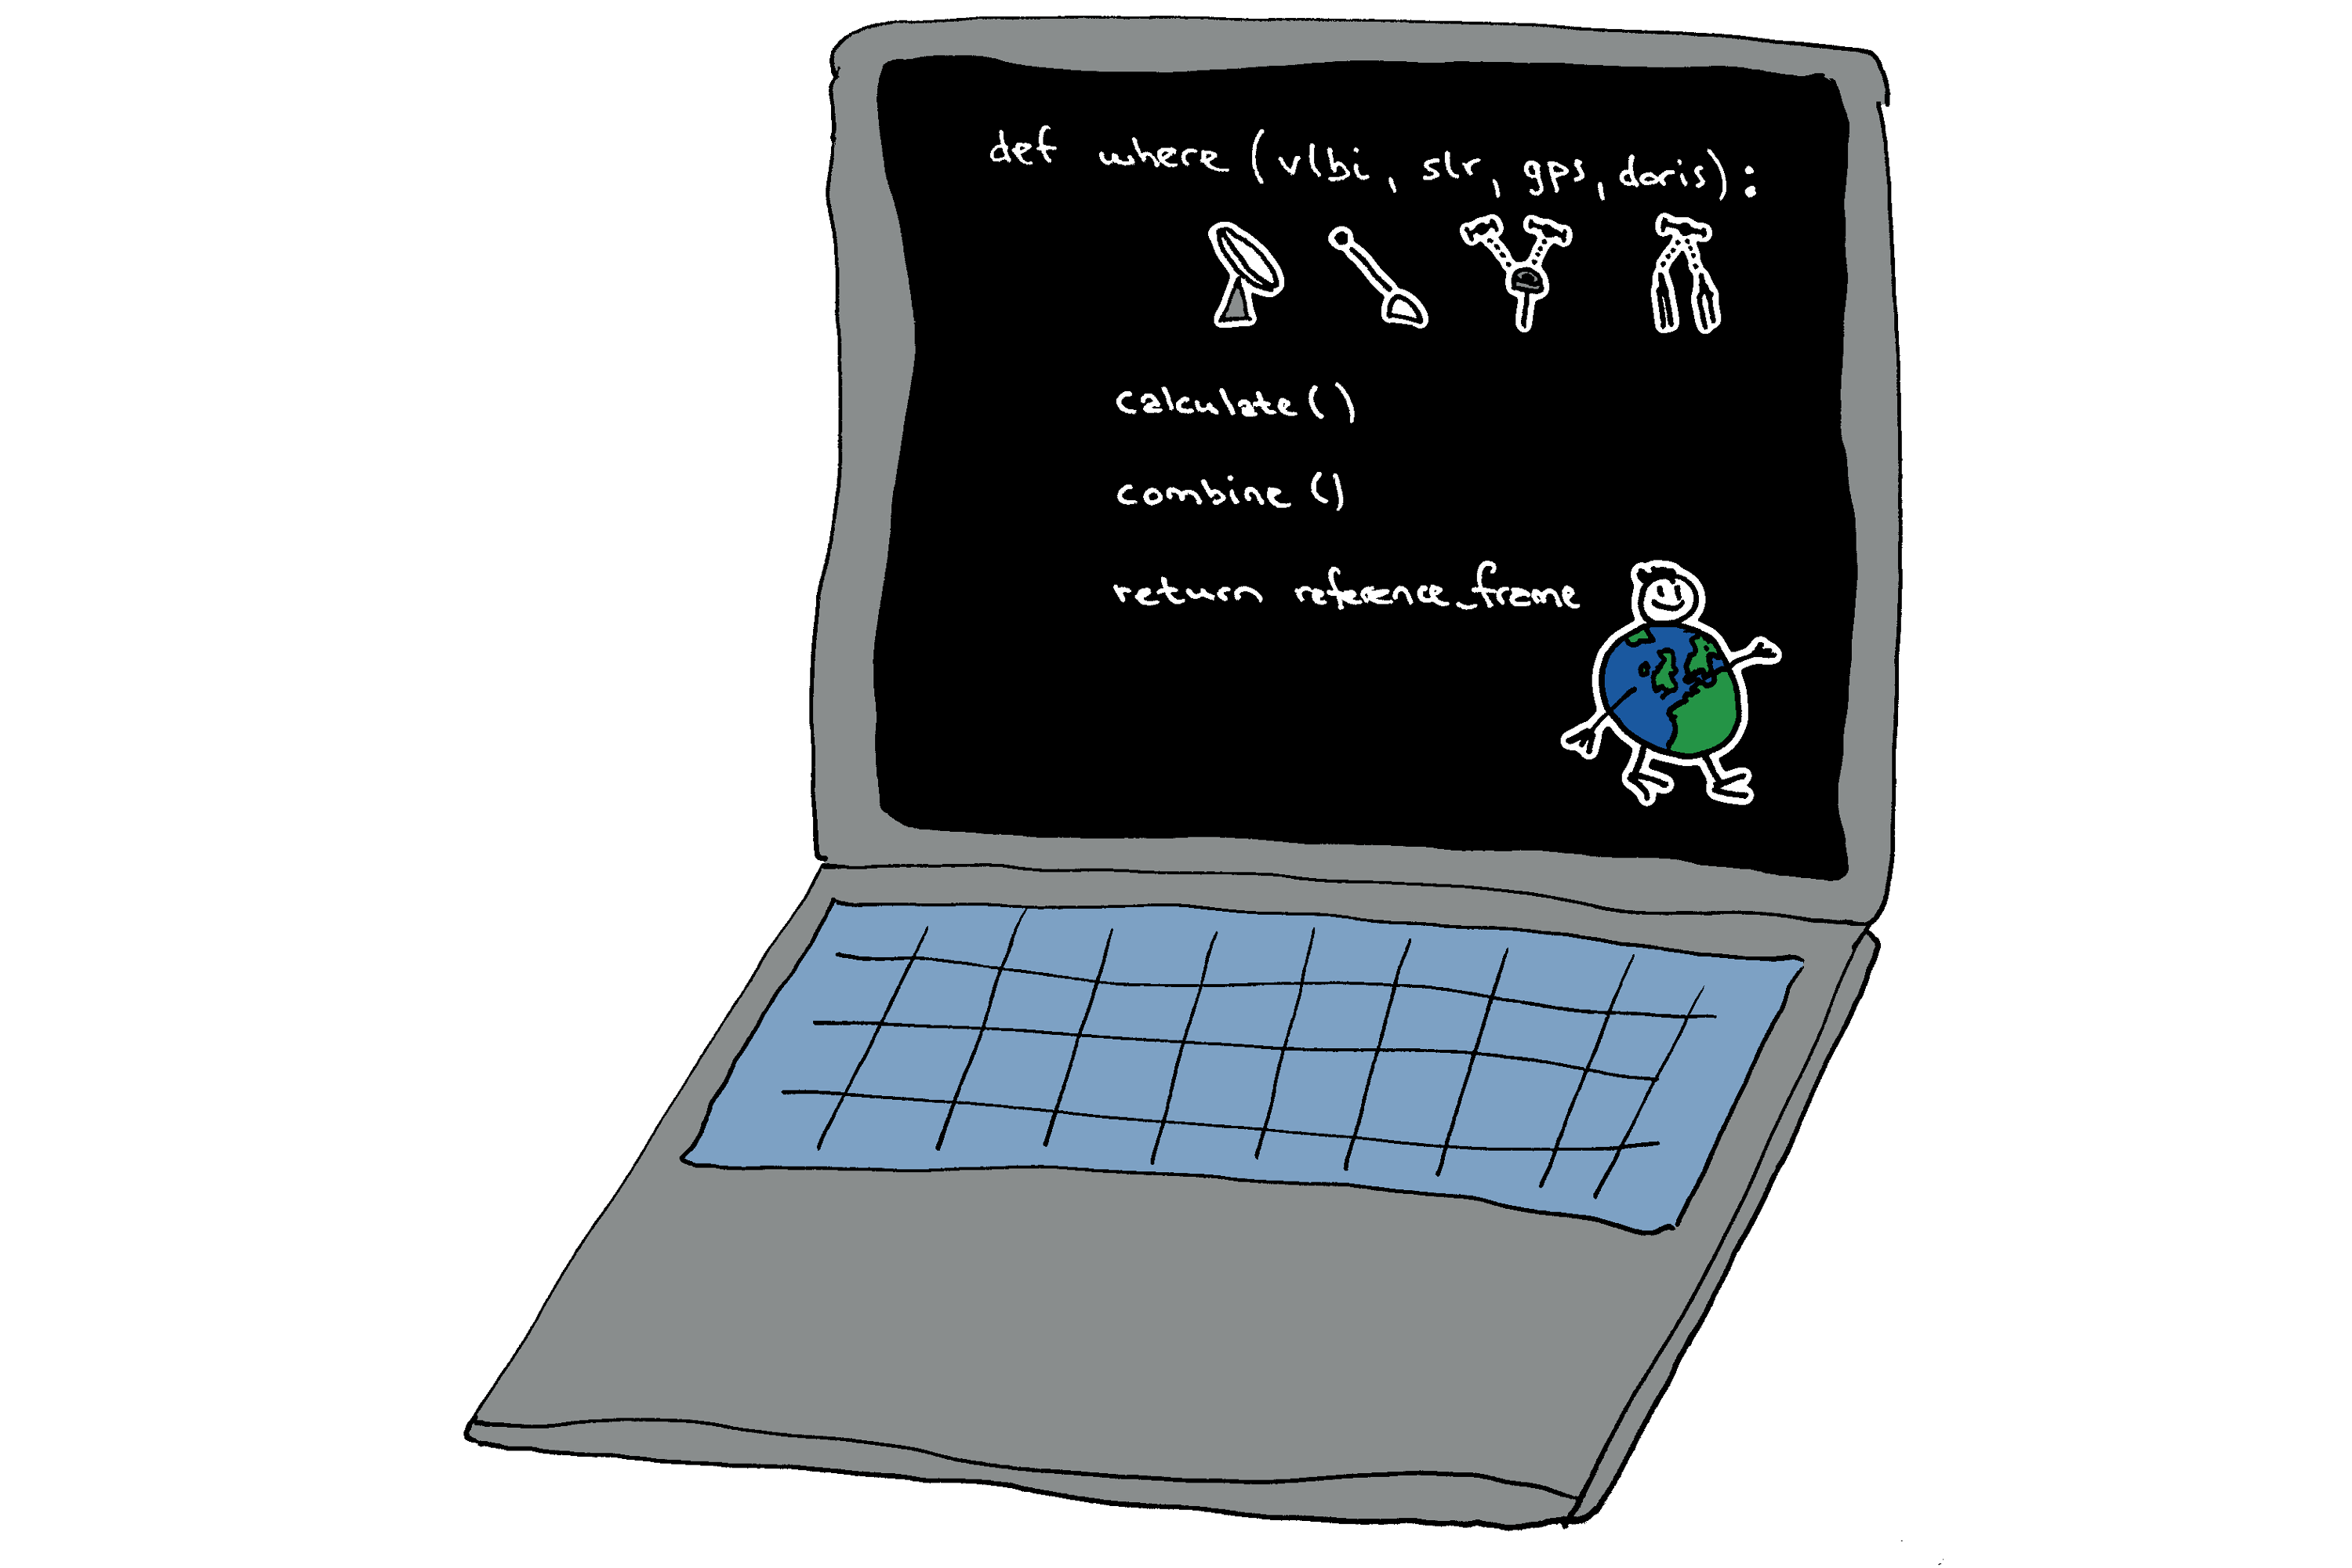
\includegraphics[width=\paperwidth]{figure/where}}

\begin{document}
\frame[plain]{\titlepage}

\part{Where}

\begin{frame}[c]{}
  
\includegraphics[width=\paperwidth]{figure/where_midgard_asgard}
\end{frame}


\begin{frame}{Analyseverktøy for Romgeodesi}
  \Where er et analyseverktøy for romgeodesi:
  \begin{itemize}[<+->]
  \item Basert på \emph{pipelines} som gjør det lett å gjenbruke modeller og
    sette opp nye analyser
  \item Inkluderer \textbf{There} for visualisering
  \item Konfigureringsmuligheter og logging for fleksible og etterprøvbare
    analyser
  \item Tilgjengelig internt og på \emph{GitHub}
  \end{itemize}
\end{frame}


\begin{frame}{Kort historie}
  \begin{description}[<+->]
  \item[T2 2015] Rammeverket for \Where ble påbegynt
  \item[Aug 2015] First light: VLBI-analyse med \Where
  \item[Høst 2015] Baneberegning/SLR-analyse i \Where påbegynt
  \item[Vår 2016] GNSS-analyse i \Where påbegynt
  \item[Vår 2017] VLBI-modellene i \Where blir testet mot andre programvarer,
    og presentert på EVGA
  \item[Mai 2017] Strategidiskusjon, ny fokus for \Where
  \item[T2 2017] SISRE-analyse i \Where påbegynt
  \item[7 juni 2018] \Where sluppet på GitHub
  \item[2018] IVS testleveranser med \Where
  \item[2018] IGN Spania bruker \Where til VLBI-analyse
  \end{description}
\end{frame}


\begin{frame}[c]{Kort historie}
  \includegraphics<1>[width=\textwidth]{figure/where_residual_1st}
  \includegraphics<2>[width=\textwidth]{figure/where_residual_2nd}
  \includegraphics<3>[width=\textwidth]{figure/where_residual_3rd}
  \includegraphics<4>[width=\textwidth]{figure/where_residual_4th}
  \includegraphics<5>[width=\textwidth]{figure/where_residual_now}
\end{frame}


\begin{frame}{Pipelines}
  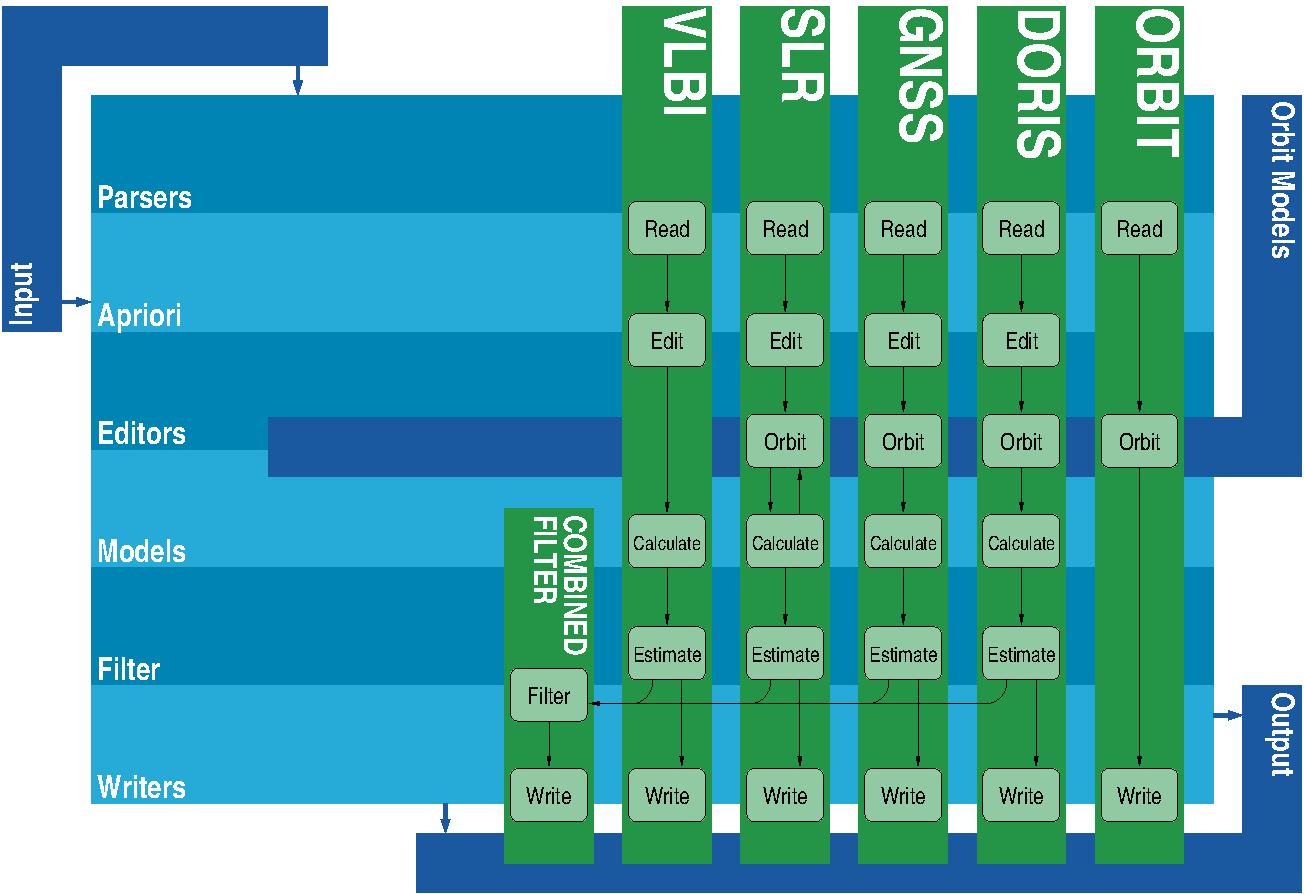
\includegraphics[width=\textwidth]{figure/code_structure}
\end{frame}


\begin{frame}{Visualisering}
  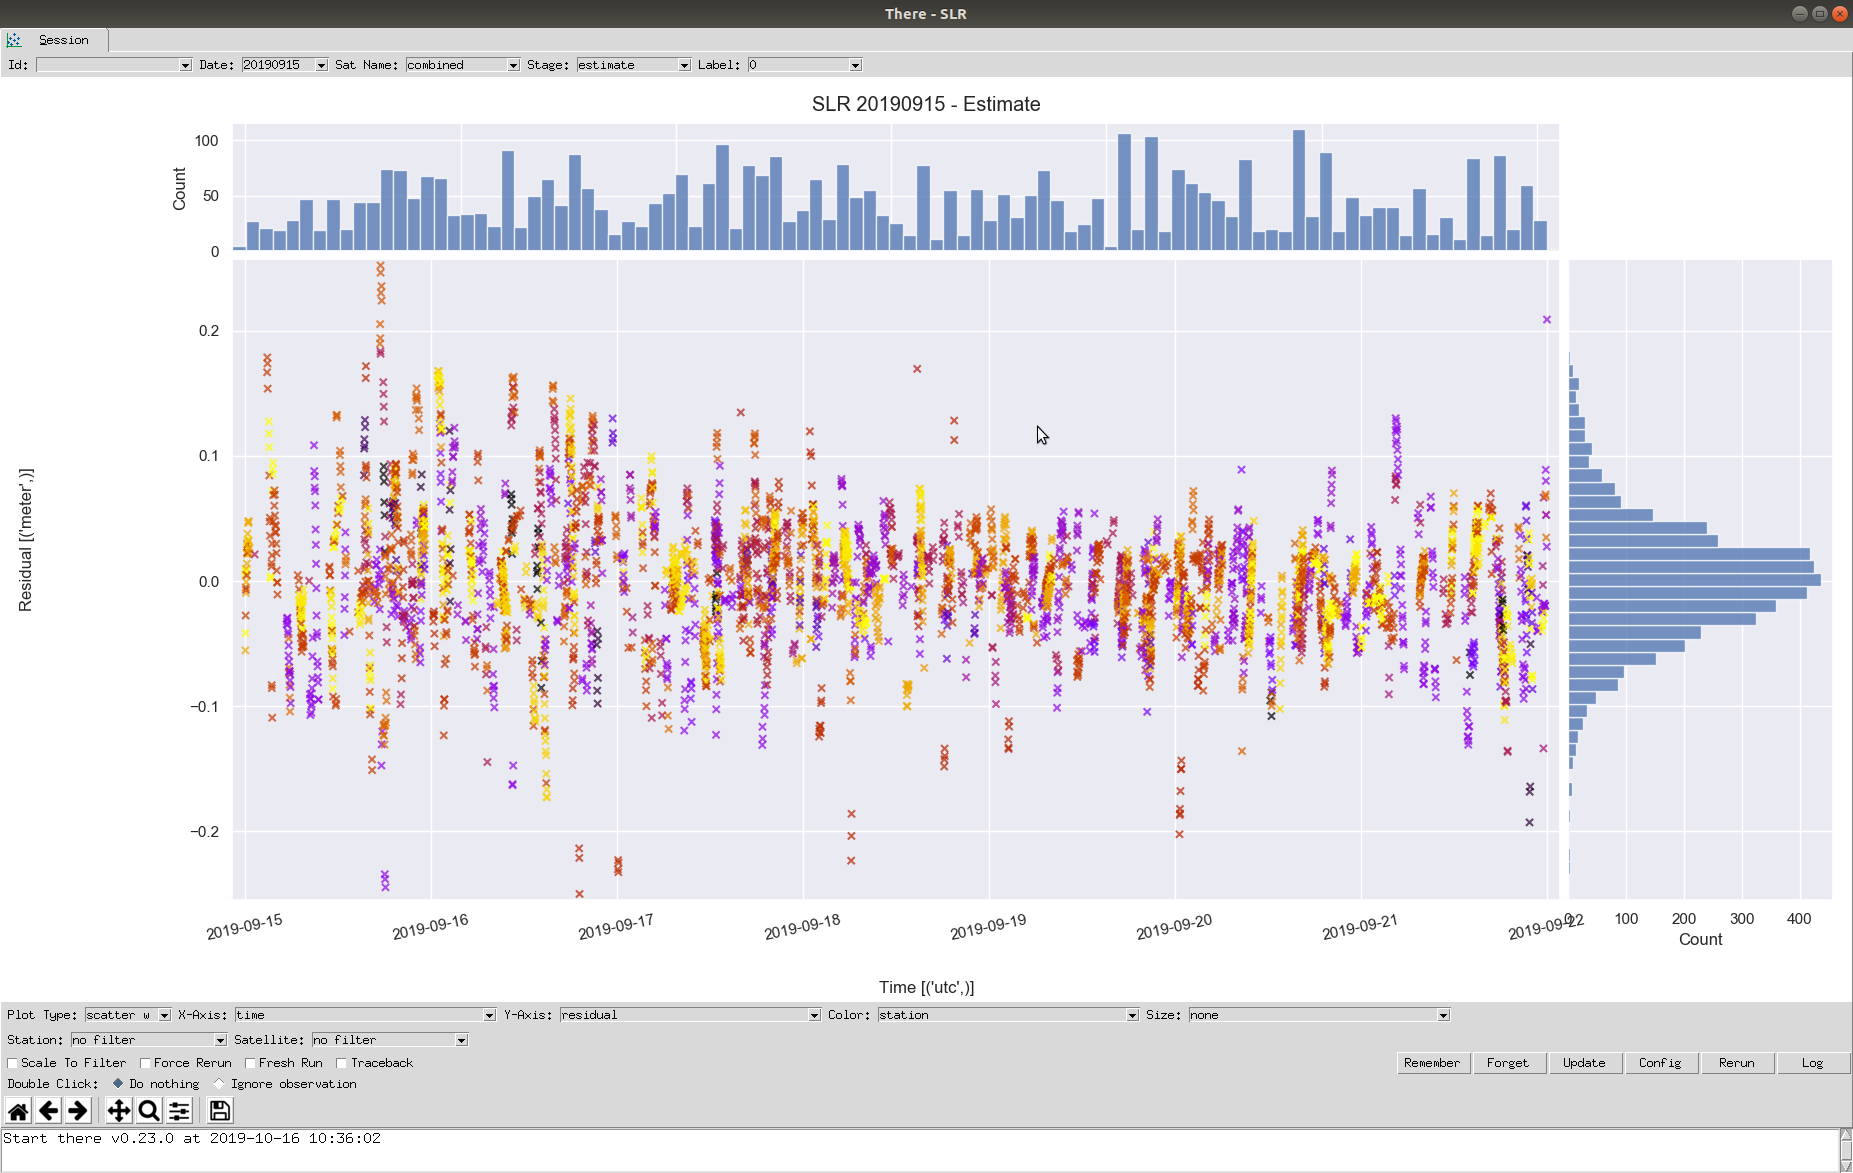
\includegraphics[width=\textwidth]{figure/there}
\end{frame}


\begin{frame}{VLBI}
  \begin{itemize}
  \item Analyser data fra VLBI-sesjoner
  \item Mål: Bli et offisielt IVS-analysesenter
  \item Bidra til beregning av jordrotasjonsparametre
  \item Bidra til forbedring av referanserammer
  \end{itemize}

  \pause
  \vfill
  \qquad $\Rightarrow$ Ann-Silje forteller mer om litt
\end{frame}


\begin{frame}{SLR}
  \begin{itemize}
  \item Analyser data fra SLR-sesjoner
  \item Mål: Bli et offisielt ILRS-analysesenter
  \item Kunne beregne satellittbaner
  \item Bidra til forbedring av referanserammer
  \end{itemize}

  \pause
  \vfill
  Status:
  \begin{itemize}
  \item Baneberegning av satelittbaner \yes
  \item Stasjonsposisjon fra SLR \yes
  \item Optimalisering av kode \yes
  \item Feilretting \no
  \item Estimering \no
  \end{itemize}
\end{frame}


\begin{frame}{GNSS -- SISRE}
  \begin{itemize}
  \item Monitorer satelittbaner for Galileo
  \item Del av GRC-MS-prosjektet
  \item Bekreftelse på at Galileosystemet leverer gode baner ut til brukerne
  \end{itemize}

  \pause
  \vfill
  \qquad $\Rightarrow$ Michael forteller mer om litt
\end{frame}


\begin{frame}{Andre pipelines}
  \Where har også noen enklere pipelines for andre oppgaver:

  \begin{itemize}
  \item GNSS -- Single Point positioning
  \item Rinex observation file manipulation
  \item Rinex navigation file manipulation
  \end{itemize}

  \pause
  \vfill
  \Where har også verktøy for automatisering av oppgaver:

  \begin{description}[concatenate]
  \item[runner] Kjøring av mange analyser på en gang
  \item[interactive] Utforsking av analysedata
  \item[concatenate] Sammensetting av analysedata
  \item[compare] Sammenligning av analysedata
  \end{description}
  
\end{frame}


\begin{frame}{Tilgjengelighet}
  \includegraphics<1>[width=\textwidth]{figure/web_where_github}
  \includegraphics<2>[width=\textwidth]{figure/web_where}
\end{frame}

\begin{frame}[fragile]{Tilgjengelighet}
I tillegg er \Where tilgjengelig fra Geodesi sin Subversion-server:

\begin{lsttermcmd}
> svn checkout http://nnriap039/repos/gdrepos/where/trunk/ where
\end{lsttermcmd}

\pause
\Where installeres med et make-script:
\begin{lsttermcmd}
> cd where
> make  
\end{lsttermcmd}

\pause
Dette fungerer på Linux. \Where kjører på Windows også, men installasjonen er
mer komplisert fordi nødvendige kompilatorer må installeres i tillegg.
  
\end{frame}

\part{Midgard}

\begin{frame}[c]{}
  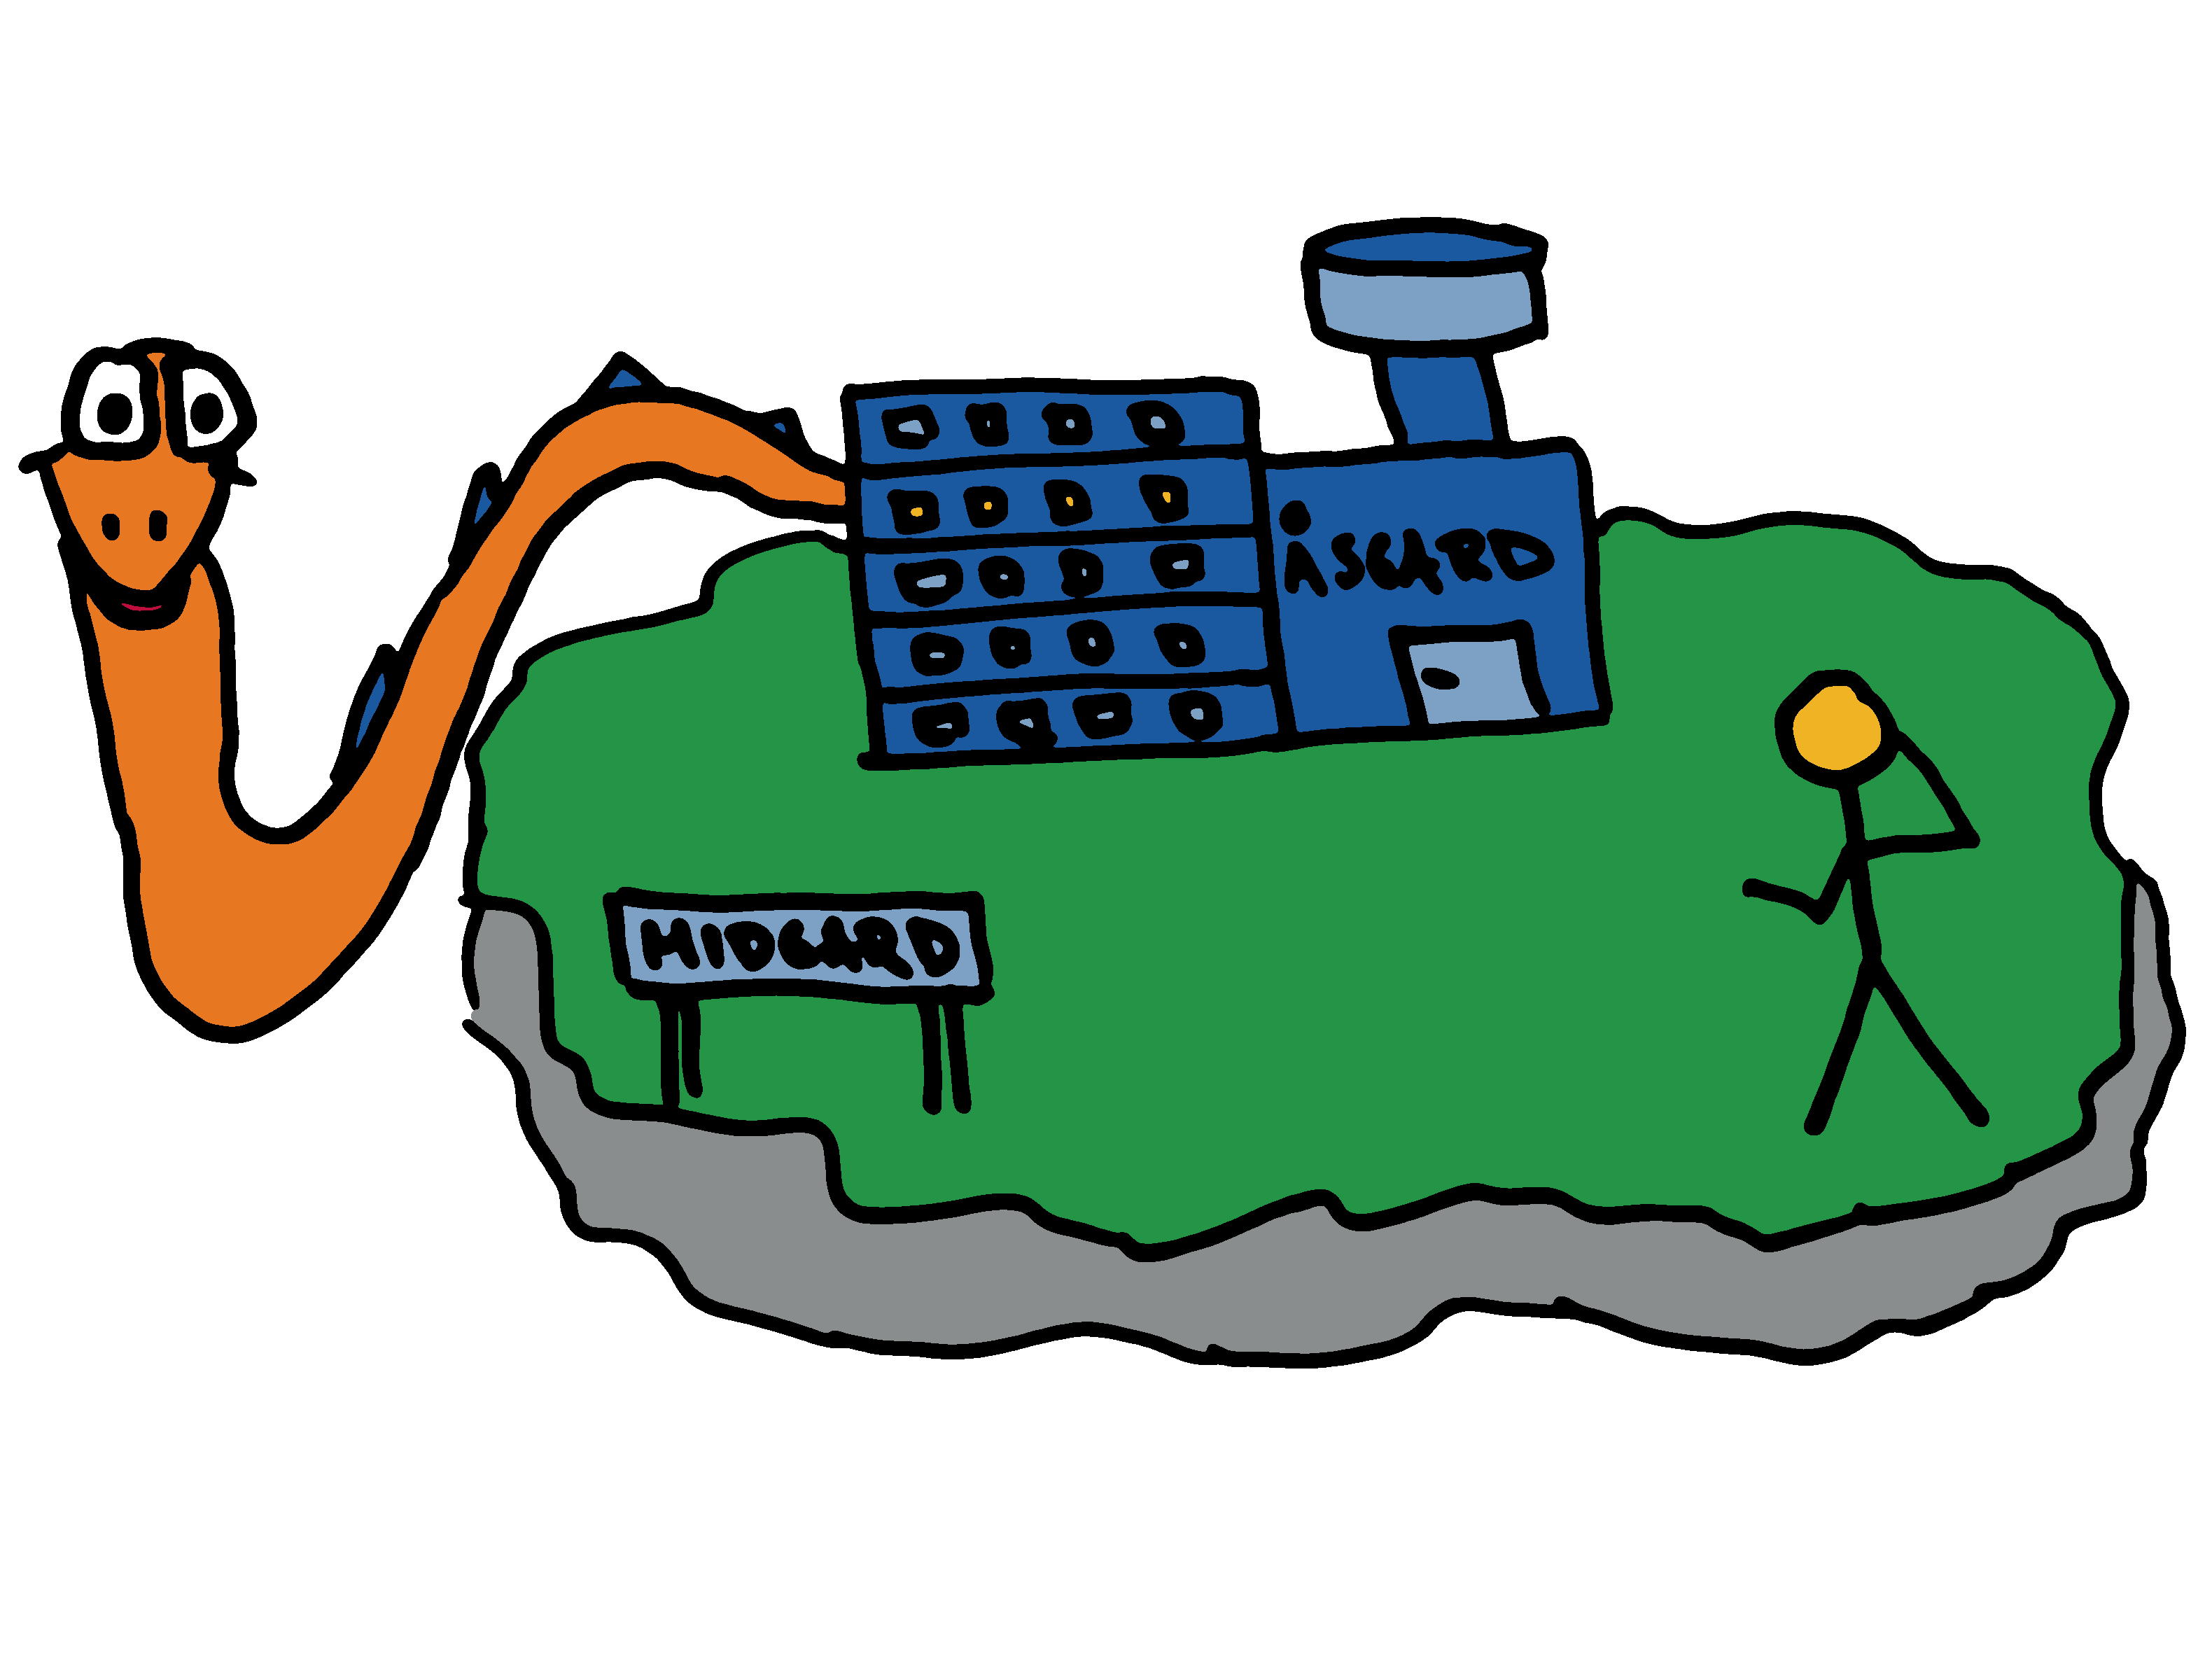
\includegraphics[width=\paperwidth]{figure/midgard_asgard}
\end{frame}

\begin{frame}{Midgard}
  En kort historietime:
  
  \begin{aquote}{Wikipedia}
    Midgard, den inngjerda verden i midten, er i norrøn mytologi menneskenes
    boplass, et av de ni hjem.
  \end{aquote}

  \pause

  \begin{aquote}{Wikipedia}
    Midgardsormen er den enorme ormen som omkranser menneskenes verden.
  \end{aquote}

  \pause

  \Midgard er det perfekte navnet på et Pythonbibliotek for geodesi!
\end{frame}


\begin{frame}{Infrastruktur}

  Pakker som kan være nyttige i mange forskjellige programmer:
  
  \begin{itemize}
  \item Konfigurasjonsfiler
  \item Logging
  \item Plug-ins
  \item Interpolasjonsrutiner
  \item Gjenbruk av C-biblioteker
  \end{itemize}
\end{frame}


\begin{frame}{Datasett}

  Egen datastruktur for håndtering av geodetiske tidsserier:
  
  \begin{itemize}
  \item Tid, med konvertering av tidsskalaer og -formater
  \item Posisjon, med konvertering mellom koordinatsystemer
  \item Hastighet
  \item Retning
  \item Tilhørende observasjonsdata
  \end{itemize}
\end{frame}


\begin{frame}[fragile]{Geodesi}

  Pakker for geodesispesifikk funksjonalitet:
  
  \begin{itemize}
  \item Lesere for forskjellige geodesifilformater
  \item Ionosfæremodeller
  \item ...
  \end{itemize}

\begin{lstpycon}
>>> from midgard import parsers
>>> p = parsers.parse_file("rinex3_header", "ande2000.17o.gz")
>>> p.header
# {'rinex_version': '3.03',
#  'file_type': 'O',
#  'sat_sys': 'G',
#  'program': 'APPL_DCB',
#  'run_by': 'NMA',
# ...}
\end{lstpycon}
\end{frame}


\begin{frame}{Tilgjengelighet}
  \includegraphics<1>[width=\textwidth]{figure/web_midgard_github}
  \includegraphics<2>[width=\textwidth]{figure/web_midgard}
  \includegraphics<3>[width=\textwidth]{figure/web_midgard_pypi}
\end{frame}

\begin{frame}[fragile]{Tilgjengelighet}
I tillegg er \Midgard tilgjengelig fra Geodesi sin Subversion-server:

\begin{lsttermcmd}
> svn checkout http://nnriap039/repos/gdrepos/midgard/trunk/ midgard
\end{lsttermcmd}

\pause
\Midgard installeres med et make-script:
\begin{lsttermcmd}
> cd midgard
> make
\end{lsttermcmd}
\end{frame}


\part{Åsgard}

\begin{frame}[c]{}
  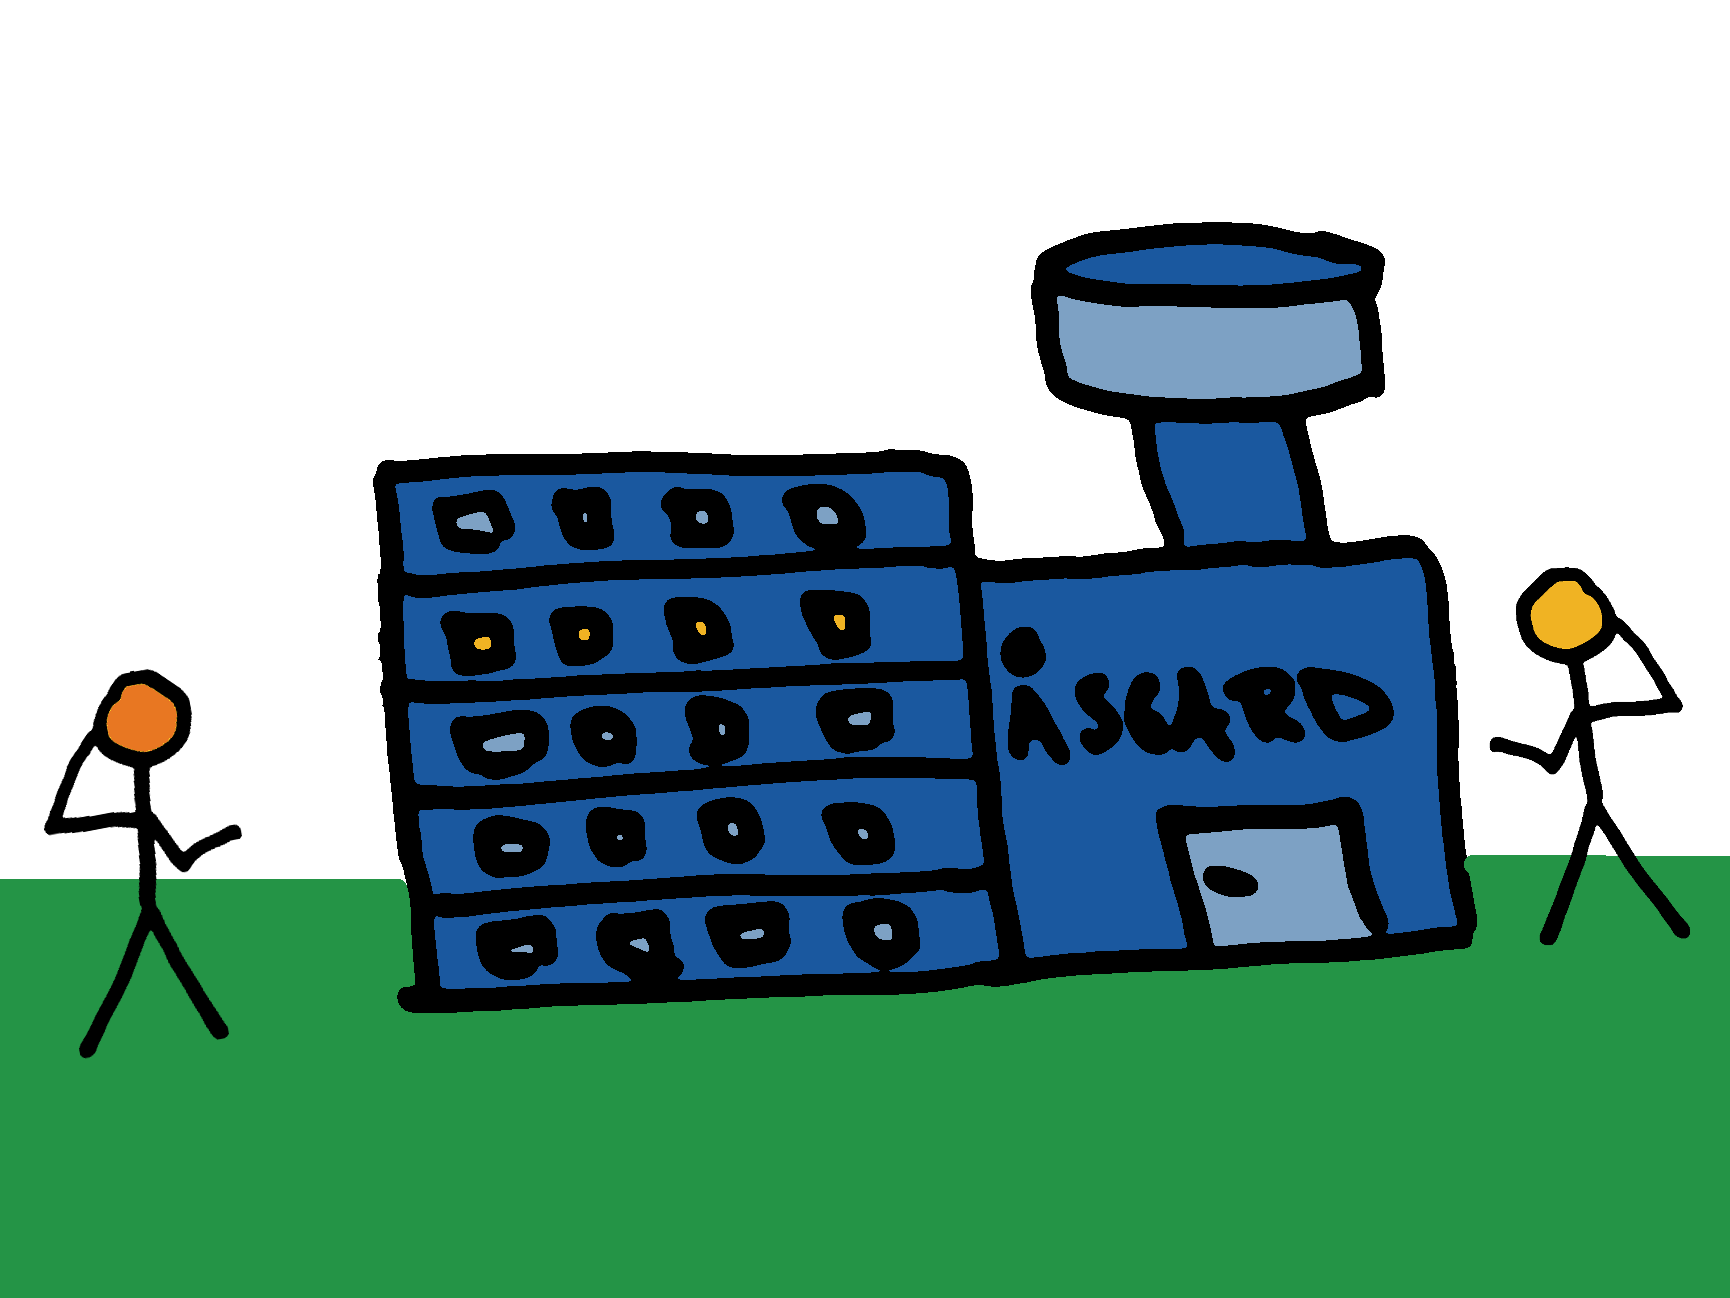
\includegraphics[width=\paperwidth]{figure/asgard}
\end{frame}

\begin{frame}{Åsgard}
  Litt mer norrøn mytologi:

  \begin{aquote}{Wikipedia}
    Åsgard er plassen som æsene bygget til seg selv, midt i Midgard, for at
    menneskene ikke skulle kjenne seg alene og forlatt.
  \end{aquote}

  \pause

  \Asgard er også et Pythonbibliotek for geodesi, men inneholder funksjonalitet
  som vi holder for oss selv!
\end{frame}


\begin{frame}{SeSite}

  \textbf{SeSite} --- Stasjonsdatabasen --- er allerede tilgjengeliggjort gjennom et API

  \begin{center}
    \includegraphics<2>[width=\textwidth]{figure/sesite01}
    \includegraphics<3>[width=\textwidth]{figure/sesite02}
    \includegraphics<4>[width=\textwidth]{figure/sesite03}
    \includegraphics<5>[width=\textwidth]{figure/sesite04}
    \includegraphics<6>[width=\textwidth]{figure/sesite05}
  \end{center}
\end{frame}
  
\begin{frame}[fragile]{SeSite}
\begin{lstpycon}
>>> from åsgard import sesite
>>> sesite.api.agencies()
# [{'id': 87332, 'agency': 'Svalsat', 'observer': 'N/A'},
#  {'id': 84516, 'agency': 'Geotrim OY', 'observer': 'N/A'},
#  ...]
\end{lstpycon}
    
\pause

\begin{lstpycon}
>>> help(sesite.api.agencies)
# Help on function agencies in module åsgard.sesite.api:
# 
# agencies(**kwargs:str) -> Dict
# Lister alle agencies, dvs firma som er ansvarlig for eller drifter en Site
\end{lstpycon}
\end{frame}

\begin{frame}[fragile]{SeSite}
\begin{lstpycon}
>>> sesite.api.sites_by_agency(agencyName="Geotrim OY")
# [{'id': 1086,
#   'active': 1,
#   'timestampRegistrated': 1369346400000,
#   'siteName': 'Utsjoki',
#   'operStatType': {'id': 27, 'operStatTypeName': 'International'},
#   'agency': {'id': 84516, 'agency': 'Geotrim OY', 'observer': 'N/A'},
#   'additionalInformation': None,
#   'siteConfigs': [{'id': 12928,
#     'fourCharId': 'UTSJ',
#     'timestampOperational': 1369346400000,
#     'timestampRemoved': None,
#     'additionalInformation': 'Lagt inn i Inngår i CPOS for at vises i norgeskart Svenske/Finske stasjoner.',
#   ...}],
# ...}]
\end{lstpycon}
\end{frame}

\begin{frame}[fragile]{SeSite}
\begin{lstpycon}
>>> sesite.api.site_by_name(siteName="andenes")
# {'id': 912,
#  'active': 1,
#  'timestampRegistrated': 977094000000,
#  'siteName': 'Andenes',
#  'operStatType': {'id': 22, 'operStatTypeName': 'Operational'},
#  'agency': {'id': 21,
#   'agency': 'Norwegian Mapping Authority',
#   'observer': 'Satref'},
#  'additionalInformation': 'Inngår i leveranse til SONEL, under namnet AND1',
#  'siteConfigs': [{'id': 11586,
#    'fourCharId': 'ANDE',
#    'timestampOperational': 977094000000,
#    'timestampRemoved': None,
#    'additionalInformation': None,
#   ...}],
# ...}]
\end{lstpycon}
\end{frame}

\begin{frame}[fragile]{Tilgjengelighet}
  \Asgard er kun tilgjengelig fra Geodesi sin Subversion-server:

  \begin{lsttermcmd}
> svn checkout http://nnriap039/repos/gdrepos/åsgard/trunk/ åsgard
  \end{lsttermcmd}
\end{frame}

\end{document}
